Primeiramente, é importante ressaltar que a elicitação remete ao significado de descobrimento. De maneira geral, cabe à elicitação a tarefa de identificar os fatos relacionados aos requisitos do sistema, de maneira a prover o mais correto e completo entendimento acerca do que é demandado pelo \emph{software} que está sendo concebido.
\\ \indent Mediante às informações apresentadas anteriormente, é necessário afirmar que a fase de levantamento de requisitos necessita de suporte para que possa ser executada com êxito.
\\ \indent Assim sendo, a partir da abordagem adotada pelo time, de natureza adaptativa, as seguintes técnicas de elicitação foram escolhidas:
\begin{itemize}
	\item{\textbf{\emph{Brainstorming}}: Técnica que consiste em reuniões para a geração de ideias, onde até as ideias não convencionais são encorajadas para a agregação do maior número de ideias possíveis para serem revisadas e escolhidas, favorecendo o surgimento de soluções criativas para o problema. No âmbito do projeto, todas as reuniões realizadas várias ideias para resolução da problemática eram apresentadas. Ao final da apresentação das sugestões, todas as propostas eram discutidas. Um momento decisivo para utilização do \emph{brainstorming} no contexto do projeto esteve atrelado à formalização dos campos que seriam solicitados no formulário de solicitação de participação do MOA e também, nas perguntas constituintes do \emph{check-list} da solicitação do MOA.}
	\item{\textbf{Prototipagem}: Técnica muito utilizada na elicitação de requisitos, pois possibilita uma visão prática, condizente ou não com o produto final baseado no seu nível de fidelidade, que facilita a interpretação concreta dos critérios a serem atingidos para a aceitação da porção da solução na qual a técnica foi utilizada. No âmbito do projeto, facilitou a interpretação concreta dos critérios a serem atingidos para a aceitação da porção da solução onde foi utilizada.
	\\ \indent Por meio das reuniões que foram realizadas, muitos aspectos eram apresentados para discussão. No momento anterior à criação da solução de BPMS, foram discutidas características da solução. Dessa maneira, foi construído um protótipo de baixa fidelidade para favorecer o entendimento.
	\begin{figure}[H]
		\centering
		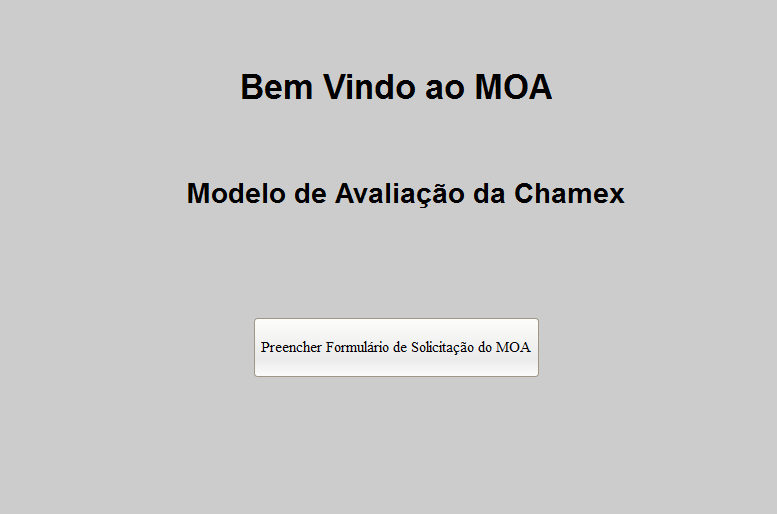
\includegraphics[scale=0.55]{prototipo_1}
		\caption[Protótipo da Página Inicial da Solução]{Protótipo da Página Inicial da Solução.}
		\label{fig:protipoum}
	\end{figure}
	\begin{figure}[H]
		\centering
		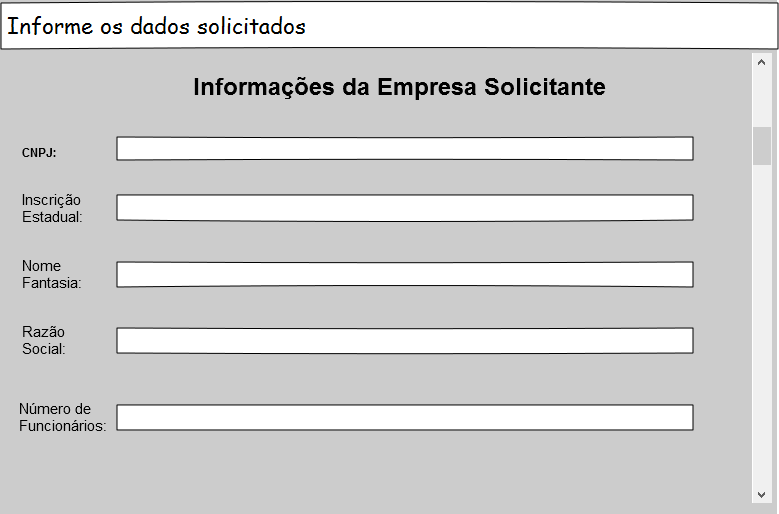
\includegraphics[scale=0.55]{prototipo_2}
		\caption[Protótipo da Primeira Página do Formulário de Inscrição]{Protótipo da Primeira Página do Formulário de Inscrição.}
		\label{fig:protipodois}
	\end{figure}
	\begin{figure}[H]
		\centering
		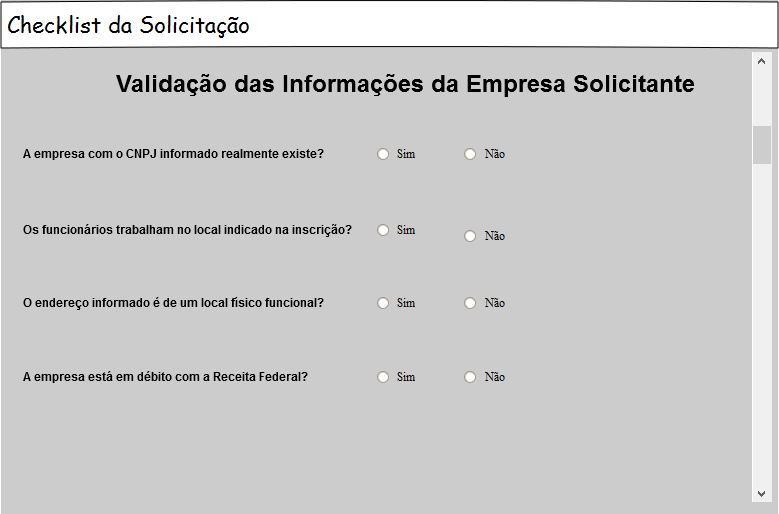
\includegraphics[scale=0.55]{prototipo_3}
		\caption[Protótipo da Página do \emph{Check-list}]{Protótipo da Página do \emph{Check-list}.}
		\label{fig:protipotres}
	\end{figure}}
\end{itemize}